%%%%%%%%%%%%%%%%%%%%%%%%%%%%%%%%%%%%%%%%%%%%%%%%%%%%%%%%%%%%%%%%%%%%%%%%%%%%%%%
% Chapter 'Absorption - 2-Propanol - ionic liquid [EMIM]+[(CF3SO2)2N]-'
%%%%%%%%%%%%%%%%%%%%%%%%%%%%%%%%%%%%%%%%%%%%%%%%%%%%%%%%%%%%%%%%%%%%%%%%%%%%%%%
\subsection{Ionic liquid [EMIM]+[(CF3SO2)2N]-}
%
%%%%%%%%%%%%%%%%%%%%%%%%%%%%%%%%%%%%%%%%%%%%%%%%%%%%%%%%%%%%%%%%%%%%%%%%%%%%%%%
%%%%%%%%%%%%%%%%%%%%%%%%%%%%%%%%%%%%%%%%%%%%%%%%%%%%%%%%%%%%%%%%%%%%%%%%%%%%%%%
\subsubsection{NrtlFixedDg - ID 1}
%
\begin{tabular}[l]{|lp{11.5cm}|}
\hline
\addlinespace

\textbf{Sorbent:} & ionic liquid \\
\textbf{Subtype:} & [EMIM]+[(CF3SO2)2N]- \\
\textbf{Refrigerant:} & 2-Propanol \\
\textbf{Equation:} & NrtlFixedDg \\
\textbf{ID:} & 1 \\
\textbf{Reference:} & Döker, Michael; Gmehling, Jürgen (2005): Measurement and prediction of vapor–liquid equilibria of ternary systems containing ionic liquids. In: Fluid Phase Equilibria 227 (2), S. 255–266. DOI: 10.1016/j.fluid.2004.11.010. \\
\textbf{Comment:} & None \\

\addlinespace
\hline
\end{tabular}
\newline

\textbf{Equation and parameters:}
\newline
%
Pressure $p$ in $\si{\pascal}$ is calculated depending on molar fraction of refrigerant in the liquid phase $x_1$ in $\si{\mole\per\mole}$, temperature $T$ in $\si{\kelvin}$, and vapor pressure $p_\mathrm{sat,1}$ in $\si{\pascal}$ by:
%
\begin{equation*}
\begin{split}
p &=& \gamma_1 x_1 p_\mathrm{sat,1} & \quad\text{, and} \\
\gamma_1 &=& \exp \left( x_2^2 \left( \tau_{21} \left( \frac{G_{21}}{x_1 + x_2 G_{21}} \right) ^2 + \tau_{12} \frac{G_{12}}{\left( x_2 + x_1 G_{12} \right) ^2}\right) \right) & \quad\text{, and} \\
G_{12} &=& \exp \left( -\alpha_{12} \tau_{12} \right) & \quad\text{, and} \\
G_{21} &=& \exp \left( -\alpha_{21} \tau_{21} \right) & \quad\text{, and} \\
\tau_{12} &=& \nicefrac{\Delta g_{12}}{R T} & \quad\text{, and} \\
\tau_{21} &=& \nicefrac{\Delta g_{21}}{R T} & \quad\text{, and} \\
x_2 &=& 1 - x_1  & \quad\text{.} \\
\end{split}
\end{equation*}
%
The parameters of the equation are:
%
\begin{longtable}[l]{lll|lll}
\toprule
\addlinespace
\textbf{Par.} & \textbf{Unit} & \textbf{Value} &	\textbf{Par.} & \textbf{Unit} & \textbf{Value} \\
\addlinespace
\midrule
\endhead

\bottomrule
\endfoot
\bottomrule
\endlastfoot
\addlinespace

$\alpha_{12}$ & - & 6.000000000e-01 & $\alpha_{21}$ & - & 6.000000000e-01 \\
$\Delta g_{12}$ & $\si{\joule\per\mole}$ & 7.795628800e+03 & $\Delta g_{21}$ & $\si{\joule\per\mole}$ & -1.003867120e+03 \\

\addlinespace\end{longtable}

\textbf{Validity:}
\newline
Equation is approximately valid for $353.15 \si{\kelvin} \leq T \leq 353.15 \si{\kelvin}$.
\newline

\textbf{Visualization:}
%
\begin{figure}[!htp]
{\noindent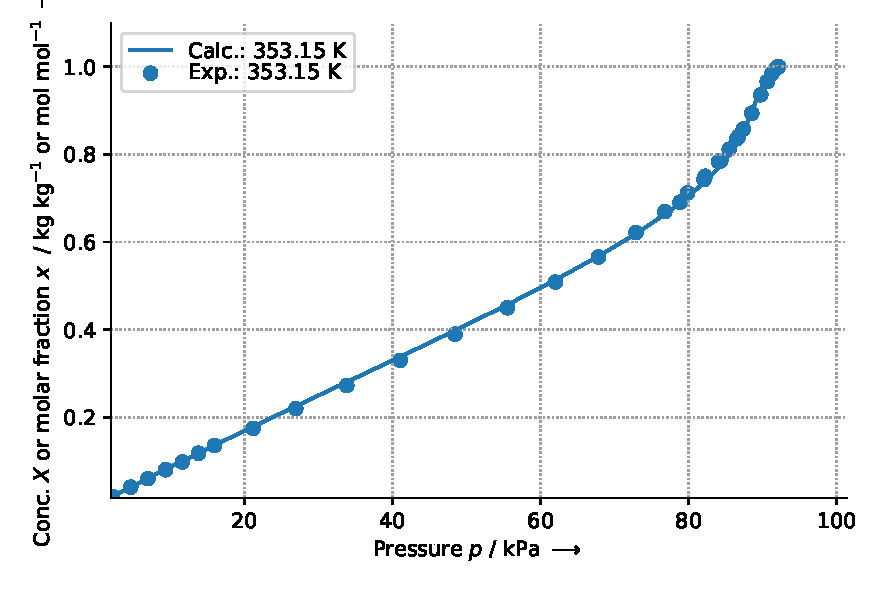
\includegraphics[height=10cm, keepaspectratio]{figs/abs/abs_2-Propanol_ionic_liquid_[EMIM]+[(CF3SO2)2N]-_NrtlFixedDg_1.pdf}}
\end{figure}
%

To generate the figure, the following refrigerant functions were selected:
\begin{itemize}
\item Vapor pressure: VaporPressure\_EoS1 - ID 1
\item Saturated liquid density: SaturatedLiquidDensity\_EoS1 - ID 1
\end{itemize}

The uncertainity of the experimental data is:
\begin{itemize}
\item Data source $\,\to\,$ Data was taken from table
\end{itemize}

The mean absolute percentage error (MAPE) between the experimental and calculated data results in 1.27\%.
\FloatBarrier
\newpage
%%%%%%%%%%%%%%%%%%%%%%%%%%%%%%%%%%%%%%%%%%%%%%%%%%%%%%%%%%%%%%%%%%%%%%%%%%%%%%%
%%%%%%%%%%%%%%%%%%%%%%%%%%%%%%%%%%%%%%%%%%%%%%%%%%%%%%%%%%%%%%%%%%%%%%%%%%%%%%%
\subsubsection{UniquacFixedDu - ID 1}
%
\begin{tabular}[l]{|lp{11.5cm}|}
\hline
\addlinespace

\textbf{Sorbent:} & ionic liquid \\
\textbf{Subtype:} & [EMIM]+[(CF3SO2)2N]- \\
\textbf{Refrigerant:} & 2-Propanol \\
\textbf{Equation:} & UniquacFixedDu \\
\textbf{ID:} & 1 \\
\textbf{Reference:} & Döker, Michael; Gmehling, Jürgen (2005): Measurement and prediction of vapor–liquid equilibria of ternary systems containing ionic liquids. In: Fluid Phase Equilibria 227 (2), S. 255–266. DOI: 10.1016/j.fluid.2004.11.010. \\
\textbf{Comment:} & None \\

\addlinespace
\hline
\end{tabular}
\newline

\textbf{Equation and parameters:}
\newline
%
Pressure $p$ in $\si{\pascal}$ is calculated depending on molar fraction of refrigerant in the liquid phase $x_1$ in $\si{\mole\per\mole}$, temperature $T$ in $\si{\kelvin}$, and vapor pressure $p_\mathrm{sat,1}$ in $\si{\pascal}$ by:
%
\begin{equation*}
\begin{split}
p &=& \gamma_1 x_1 p_\mathrm{sat,1} & \quad\text{, and} \\
\gamma_1 &=& \exp \left( \ln \left( \nicefrac{\Phi_1}{x_1} \right) + q_1 \nicefrac{z}{2} \ln \left( \nicefrac{\Theta_1}{\Phi_1} \right) + l_1 - \nicefrac{\Phi_1}{x_2} \left( x_1 l_1 + x_2 l_2 \right) + \Gamma \right) & \quad\text{, and} \\
\Gamma &=& - q_1 \ln \left( \Theta_1 + \Theta_2 \tau_{21} \right) + q_1 - q_1 \left( \frac{\Theta_1}{\Theta_1 + \Theta_2 \tau_{21}} + \frac{\Theta_2 \tau_{12}}{\Theta_1 \tau_{12} + \Theta_2} \right) & \quad\text{, and} \\
\tau_{ij} &=& \exp \left( \nicefrac{\Delta u_{ij}}{R T} \right) & \quad\text{, and} \\
l_i &=& \nicefrac{z}{2} \left( r_i - q_i \right) \left(r_i - 1 \right) & \quad\text{, and} \\
\Theta_i &=& \frac{q_i x_i}{\sum_{j=1}^{2} q_j x_j} & \quad\text{, and} \\
\Phi_i &=& \frac{r_i x_i}{\sum_{j=1}^{2} r_j x_j} & \quad\text{, and} \\
x_2 &=& 1 - x_1  & \quad\text{.} \\
\end{split}
\end{equation*}
%
The parameters of the equation are:
%
\begin{longtable}[l]{lll|lll}
\toprule
\addlinespace
\textbf{Par.} & \textbf{Unit} & \textbf{Value} &	\textbf{Par.} & \textbf{Unit} & \textbf{Value} \\
\addlinespace
\midrule
\endhead

\bottomrule
\endfoot
\bottomrule
\endlastfoot
\addlinespace

$\Delta u_{12}$ & $\si{\joule\per\mole}$ & 1.536364800e+03 & $\Delta u_{21}$ & $\si{\joule\per\mole}$ & -2.923904720e+02 \\
$r_{1}$ & - & 2.779100000e+00 & $r_{2}$ & - & 9.890000000e+00 \\
$q_{1}$ & - & 2.508000000e+00 & $q_{2}$ & - & 8.780000000e+00 \\
$z$ & - & 1.000000000e+01 & & &  \\

\addlinespace\end{longtable}

\textbf{Validity:}
\newline
Equation is approximately valid for $353.15 \si{\kelvin} \leq T \leq 353.15 \si{\kelvin}$.
\newline

\textbf{Visualization:}
%
\begin{figure}[!htp]
{\noindent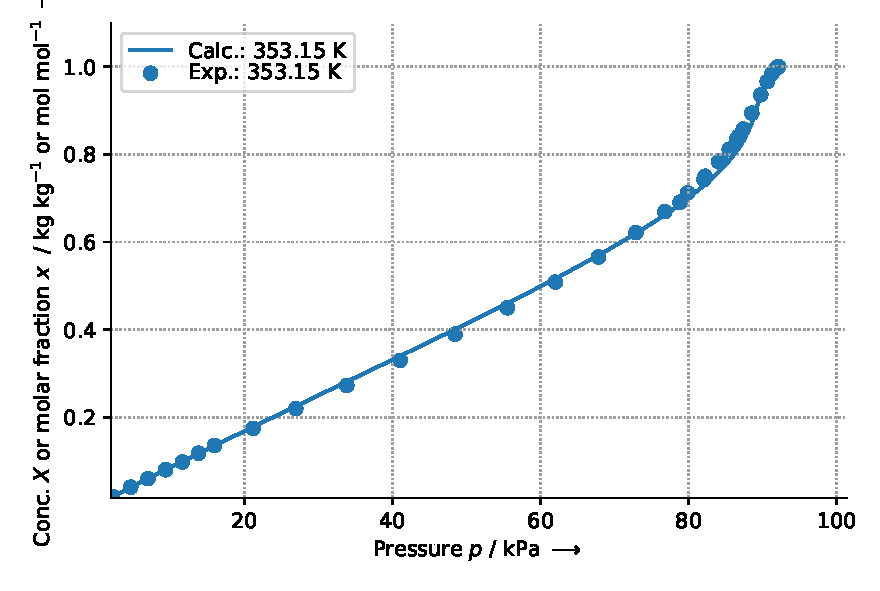
\includegraphics[height=10cm, keepaspectratio]{figs/abs/abs_2-Propanol_ionic_liquid_[EMIM]+[(CF3SO2)2N]-_UniquacFixedDu_1.pdf}}
\end{figure}
%

To generate the figure, the following refrigerant functions were selected:
\begin{itemize}
\item Vapor pressure: VaporPressure\_EoS1 - ID 1
\item Saturated liquid density: SaturatedLiquidDensity\_EoS1 - ID 1
\end{itemize}

The uncertainity of the experimental data is:
\begin{itemize}
\item Data source $\,\to\,$ Data was taken from table
\end{itemize}

The mean absolute percentage error (MAPE) between the experimental and calculated data results in 1.62\%.
\FloatBarrier
\newpage
%%%%%%%%%%%%%%%%%%%%%%%%%%%%%%%%%%%%%%%%%%%%%%%%%%%%%%%%%%%%%%%%%%%%%%%%%%%%%%%
%%%%%%%%%%%%%%%%%%%%%%%%%%%%%%%%%%%%%%%%%%%%%%%%%%%%%%%%%%%%%%%%%%%%%%%%%%%%%%%
\subsubsection{UniquacFixedDu - ID 2}
%
\begin{tabular}[l]{|lp{11.5cm}|}
\hline
\addlinespace

\textbf{Sorbent:} & ionic liquid \\
\textbf{Subtype:} & [EMIM]+[(CF3SO2)2N]- \\
\textbf{Refrigerant:} & 2-Propanol \\
\textbf{Equation:} & UniquacFixedDu \\
\textbf{ID:} & 2 \\
\textbf{Reference:} & Kato, Ryo; Gmehling, Jürgen (2005): Measurement and correlation of vapor–liquid equilibria of binary systems containing the ionic liquids [EMIM][(CF3SO2)2N], [BMIM][(CF3SO2)2N], [MMIM][(CH3)2PO4] and oxygenated organic compounds respectively water. In: Fluid Phase Equilibria 231 (1), S. 38–43. DOI: 10.1016/j.fluid.2005.01.002. \\
\textbf{Comment:} & None \\

\addlinespace
\hline
\end{tabular}
\newline

\textbf{Equation and parameters:}
\newline
%
Pressure $p$ in $\si{\pascal}$ is calculated depending on molar fraction of refrigerant in the liquid phase $x_1$ in $\si{\mole\per\mole}$, temperature $T$ in $\si{\kelvin}$, and vapor pressure $p_\mathrm{sat,1}$ in $\si{\pascal}$ by:
%
\begin{equation*}
\begin{split}
p &=& \gamma_1 x_1 p_\mathrm{sat,1} & \quad\text{, and} \\
\gamma_1 &=& \exp \left( \ln \left( \nicefrac{\Phi_1}{x_1} \right) + q_1 \nicefrac{z}{2} \ln \left( \nicefrac{\Theta_1}{\Phi_1} \right) + l_1 - \nicefrac{\Phi_1}{x_2} \left( x_1 l_1 + x_2 l_2 \right) + \Gamma \right) & \quad\text{, and} \\
\Gamma &=& - q_1 \ln \left( \Theta_1 + \Theta_2 \tau_{21} \right) + q_1 - q_1 \left( \frac{\Theta_1}{\Theta_1 + \Theta_2 \tau_{21}} + \frac{\Theta_2 \tau_{12}}{\Theta_1 \tau_{12} + \Theta_2} \right) & \quad\text{, and} \\
\tau_{ij} &=& \exp \left( \nicefrac{\Delta u_{ij}}{R T} \right) & \quad\text{, and} \\
l_i &=& \nicefrac{z}{2} \left( r_i - q_i \right) \left(r_i - 1 \right) & \quad\text{, and} \\
\Theta_i &=& \frac{q_i x_i}{\sum_{j=1}^{2} q_j x_j} & \quad\text{, and} \\
\Phi_i &=& \frac{r_i x_i}{\sum_{j=1}^{2} r_j x_j} & \quad\text{, and} \\
x_2 &=& 1 - x_1  & \quad\text{.} \\
\end{split}
\end{equation*}
%
The parameters of the equation are:
%
\begin{longtable}[l]{lll|lll}
\toprule
\addlinespace
\textbf{Par.} & \textbf{Unit} & \textbf{Value} &	\textbf{Par.} & \textbf{Unit} & \textbf{Value} \\
\addlinespace
\midrule
\endhead

\bottomrule
\endfoot
\bottomrule
\endlastfoot
\addlinespace

$\Delta u_{12}$ & $\si{\joule\per\mole}$ & 1.536400000e+03 & $\Delta u_{21}$ & $\si{\joule\per\mole}$ & -2.924000000e+02 \\
$r_{1}$ & - & 2.789000000e+00 & $r_{2}$ & - & 9.890000000e+00 \\
$q_{1}$ & - & 2.508000000e+00 & $q_{2}$ & - & 8.780000000e+00 \\
$z$ & - & 1.000000000e+01 & & &  \\

\addlinespace\end{longtable}

\textbf{Validity:}
\newline
Equation is approximately valid for $353.15 \si{\kelvin} \leq T \leq 353.15 \si{\kelvin}$.
\newline

\textbf{Visualization:}
%
\begin{figure}[!htp]
{\noindent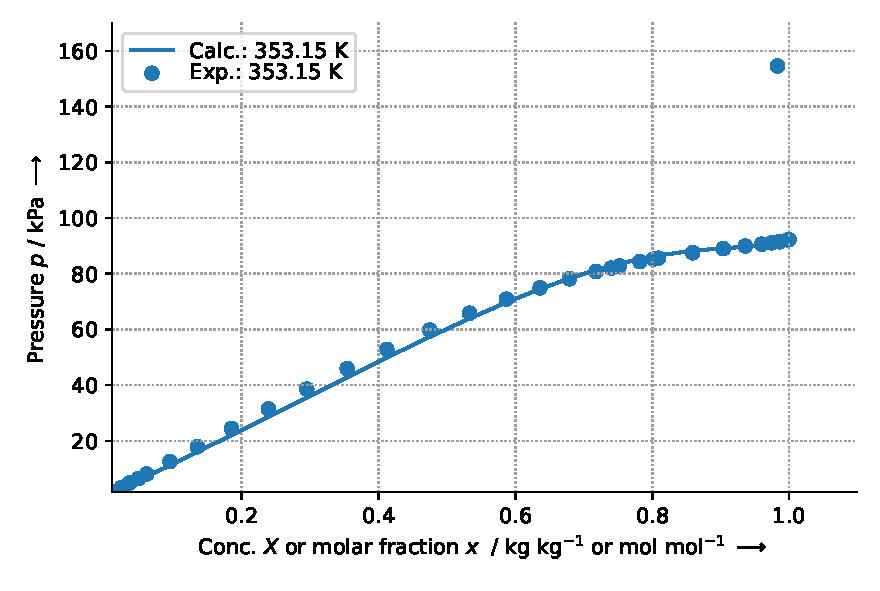
\includegraphics[height=10cm, keepaspectratio]{figs/abs/abs_2-Propanol_ionic_liquid_[EMIM]+[(CF3SO2)2N]-_UniquacFixedDu_2.pdf}}
\end{figure}
%

To generate the figure, the following refrigerant functions were selected:
\begin{itemize}
\item Vapor pressure: VaporPressure\_EoS1 - ID 1
\item Saturated liquid density: SaturatedLiquidDensity\_EoS1 - ID 1
\end{itemize}

The uncertainity of the experimental data is:
\begin{itemize}
\item Data source $\,\to\,$ Data was taken from table
\end{itemize}

The mean absolute percentage error (MAPE) between the experimental and calculated data results in 5.7\%.
\FloatBarrier
\newpage
%%%%%%%%%%%%%%%%%%%%%%%%%%%%%%%%%%%%%%%%%%%%%%%%%%%%%%%%%%%%%%%%%%%%%%%%%%%%%%%
%%%%%%%%%%%%%%%%%%%%%%%%%%%%%%%%%%%%%%%%%%%%%%%%%%%%%%%%%%%%%%%%%%%%%%%%%%%%%%%
\subsubsection{WilsonFixedDl - ID 1}
%
\begin{tabular}[l]{|lp{11.5cm}|}
\hline
\addlinespace

\textbf{Sorbent:} & ionic liquid \\
\textbf{Subtype:} & [EMIM]+[(CF3SO2)2N]- \\
\textbf{Refrigerant:} & 2-Propanol \\
\textbf{Equation:} & WilsonFixedDl \\
\textbf{ID:} & 1 \\
\textbf{Reference:} & Döker, Michael; Gmehling, Jürgen (2005): Measurement and prediction of vapor–liquid equilibria of ternary systems containing ionic liquids. In: Fluid Phase Equilibria 227 (2), S. 255–266. DOI: 10.1016/j.fluid.2004.11.010. \\
\textbf{Comment:} & None \\

\addlinespace
\hline
\end{tabular}
\newline

\textbf{Equation and parameters:}
\newline
%
Pressure $p$ in $\si{\pascal}$ is calculated depending on molar fraction of refrigerant in the liquid phase $x_1$ in $\si{\mole\per\mole}$, temperature $T$ in $\si{\kelvin}$, molar volumes of both components ($v_1$ and $v_2$) in $\si{\cubic\meter\per\mole}$, and vapor pressure $p_\mathrm{sat,1}$ in $\si{\pascal}$. If molar volumes less than zero are used as function arguements, constant molar volumes given by parameter record are used. Equilibrium equation is given by:
%
\begin{equation*}
\begin{split}
p &=& \gamma_1 x_1 p_\mathrm{sat,1} & \quad\text{, and} \\
\gamma_1 &=& \exp \left( - \ln \left( x_1 + \Lambda_{12} x_2 \right) + x_2 \left( \frac{\Lambda_{12}}{x_1 + \Lambda_{12} x_2} - \frac{\Lambda_{21}}{x_2 + \Lambda_{21} x_1} \right) \right) & \quad\text{, and} \\
\Lambda_{12} &=& \begin{cases} \nicefrac{v_2}{v_1} \exp \left( - \nicefrac{\Delta\lambda_{12}}{R T} \right) & \quad \text{if } \Lambda_{12}^{*} = 0 \\ \Lambda_{12}^{*}  & \quad \text{else} \end{cases}  & \quad\text{, and} \\
\Lambda_{21} &=& \begin{cases} \nicefrac{v_1}{v_2} \exp \left( - \nicefrac{\Delta\lambda_{21}}{R T} \right) & \quad \text{if } \Lambda_{21}^{*} = 0 \\ \Lambda_{21}^{*}  & \quad \text{else} \end{cases}  & \quad\text{, and} \\
x_2 &=& 1 - x_1  & \quad\text{.} \\
\end{split}
\end{equation*}
%
The parameters of the equation are:
%
\begin{longtable}[l]{lll|lll}
\toprule
\addlinespace
\textbf{Par.} & \textbf{Unit} & \textbf{Value} &	\textbf{Par.} & \textbf{Unit} & \textbf{Value} \\
\addlinespace
\midrule
\endhead

\bottomrule
\endfoot
\bottomrule
\endlastfoot
\addlinespace

$\Lambda_{12}^{*}$ & - & 0.000000000e+00 & $\Lambda_{21}^{*}$ & - & 0.000000000e+00 \\
$\Delta\lambda_{12}$ & $\si{\joule\per\mole}$ & 1.189343840e+03 & $\Delta\lambda_{21}$ & $\si{\joule\per\mole}$ & 1.673600000e+04 \\
$v_1$ & $\si{\cubic\meter\per\mole}$ & 7.692000000e+01 & $v_2$ & $\si{\cubic\meter\per\mole}$ & 2.445800000e+02 \\

\addlinespace\end{longtable}

\textbf{Validity:}
\newline
Equation is approximately valid for $353.15 \si{\kelvin} \leq T \leq 353.15 \si{\kelvin}$.
\newline

\textbf{Visualization:}
%
\begin{figure}[!htp]
{\noindent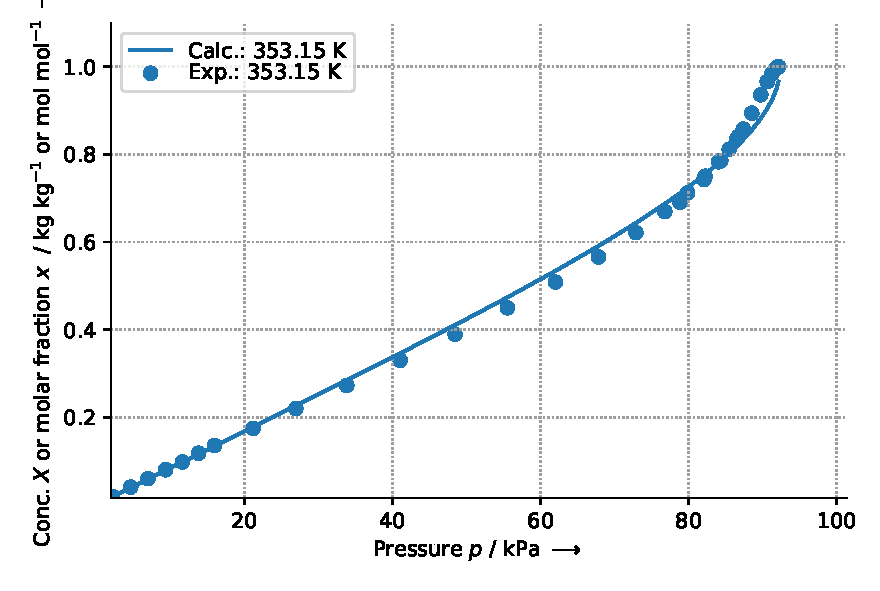
\includegraphics[height=10cm, keepaspectratio]{figs/abs/abs_2-Propanol_ionic_liquid_[EMIM]+[(CF3SO2)2N]-_WilsonFixedDl_1.pdf}}
\end{figure}
%

To generate the figure, the following refrigerant functions were selected:
\begin{itemize}
\item Vapor pressure: VaporPressure\_EoS1 - ID 1
\item Saturated liquid density: SaturatedLiquidDensity\_EoS1 - ID 1
\end{itemize}

The uncertainity of the experimental data is:
\begin{itemize}
\item Data source $\,\to\,$ Data was taken from table
\end{itemize}

The mean absolute percentage error (MAPE) between the experimental and calculated data results in 3.02\%.
\FloatBarrier
\newpage
%%%%%%%%%%%%%%%%%%%%%%%%%%%%%%%%%%%%%%%%%%%%%%%%%%%%%%%%%%%%%%%%%%%%%%%%%%%%%%%
